\documentclass{beamer}

\usetheme{default}

\title{HORIZON-WIDERA-2025-01-ACCESS-01}
\author{NTUA/DSO}
\date{\today}

\begin{document}

% Title Slide
\begin{frame}
  \titlepage
\end{frame}

% Slide 1
\begin{frame}{Proposal}

Call:
\vspace{1cm}
European Excellence Initiative (EEI)
\href{https://ec.europa.eu/info/funding-tenders/opportunities/portal/screen/opportunities/topic-details/HORIZON-WIDERA-2025-01-ACCESS-01}{HORIZON-WIDERA-2025-01-ACCESS-01}
Type of funding: CSA / Action Grant Budget-Based

\vspace{1cm}

  \begin{itemize}
    \item Duration: Up to five years
    \item Budget: Up to 5Mil., at least 51\% must be consumed by Widening Partners!
    \item Deadline: 20 November 2025 17:00:00 Brussels time
    \item Indicative Number of Grants: 27
  \end{itemize}
\end{frame}

% Slide 2
\begin{frame}{Eligibility conditions}

In order to achieve the expected outcomes, \textbf{participation as coordinators to
the call is limited to legal entities established in Widening countries}.

\vspace{1cm}

Applications must be submitted by a consortium, including as
beneficiaries, \textbf{at least three independent legal entities, in three different EU
Member States or Horizon Europe Associated Countries}.
\end{frame}

\begin{frame}{Consortium}
\begin{columns}

  \begin{column}{0.48\textwidth}
    \textbf{Widening Partners}

    \begin{enumerate}
      \item National Technical University of Athens,
      \item Technical University of Crete,
      \item University of West Attica (UNIWA),
      \item TotalView (Greece),
      \item Akdeniz University / Faculty of Science, Department of Space Sciences and Technologies,
      % \item Geodetic Observatory Pency
      \item Research Institute of Geodesy, Topography and Cartography, v.v.i
    \end{enumerate}
  \end{column}

  \begin{column}{0.48\textwidth}
    % Right column content
    \textbf{Expert Partners}
    \begin{enumerate}
    \item GFZ Helmholtz Centre for Geosciences, Germany
    \item Institut de Physique du Globe de Paris (IPGP), France
    \item Collecte Localisation Satellites (CLS), France
    \item Chalmers University of Technology, Sweden
    \end{enumerate}
  \end{column}

\end{columns}
\end{frame}

\begin{frame}{Outcome \& Objectives (1/4)}
The EU higher education system is quite inclusive and provides a high level of
education and training to a significant portion of its young people. However, 
\textbf{there are very large differences among European universities}, and 
some perform very well in many respects. \textbf{This action addresses this 
challenge by dedicated measures to reduce these disparities by
raising the overall level of excellence of research undertaken in higher education entities}.
\end{frame}

\begin{frame}{Outcome \& Objectives (2/4)}
  
\footnotesize
\begin{itemize}
  \item \textbf{Raise excellence in science and in knowledge valorisation} through deeper and
geographically inclusive strategic cooperation in alliances of higher education
institutions, such as – but not limited to – European Universities alliances selected under
Erasmus+, with a center of gravity in Widening countries;
  \item \textbf{Improve global competitiveness and visibility of Europe’s higher education institutions},
creating critical mass in key strategic areas stipulated in the political guidelines for the
next European Commission published in July 202428 such as the Clean Industrial Deal,
the Energy Union, digital tech diffusion, artificial intelligence, the upcoming European
Life Science strategy, Union of Skills, etc.;
  \item \textbf{Improve researchers career opportunities} in line with the ERA policy agenda 2022-24,
promoting a balanced circulation of talents, fair and modern research assessment
practices in line with the Agreement on Reforming Research Assessment29, \textbf{diversity,
gender equality and inclusiveness, use of open science practices as well as the
acquisition of transferable skills}.
\end{itemize}
\end{frame}

\begin{frame}{Outcome \& Objectives (3/4)}
  
\footnotesize
\begin{itemize}
\item \textbf{Modernisation and upgrade} of higher education institutions in the R\&I dimension,
through integrated \textbf{collaboration} between institutions and with other actors in local
ecosystems and/or internationally;
\item Mainstreamed \textbf{culture of excellence} in science and knowledge valorisation amongst
higher education institutions, and particularly in less research-intensive institutions and
countries, \textbf{in particular Widening countries};
\item Accelerated \textbf{institutional reforms} in the R\&I dimension and \textbf{strengthened R\&I capacities}
in higher education institutions, notably those located in Widening countries, in
particular leading to better research careers including in non-academic sectors;
\item Strengthened \textbf{digital skills and capacities} including artificial intelligence of the R\&I
dimension of the higher education sector;
\item Increased \textbf{global competitiveness} and critical mass of research in the European higher
education system;
\item Contribution to implementation of the relevant ERA Policy Agenda 2022-24 actions in
higher education sector 
\end{itemize}
\end{frame}

\begin{frame}{Outcome \& Objectives (4/4)}
  
\begin{itemize}
\item Develop closer cooperation with economic and industrial partners within local and
regional innovation ecosystems, academic researchers and support staff 
\item Trained in knowledge valorisation, entrepreneurship, access to finance
\item Activities need to focus on research and innovation conducted in the higher education sector.
\item Educational activities such as Master or doctoral programmes are out of scope of this call.
\item Expenditures for research and innovation activities cannot exceed a maximum of 20\% of the total 
budget and need to be presented in a dedicated and distinct work package in the proposal.
\end{itemize}
\end{frame}

\begin{frame}{CoE in Space Geodesy}
What are we proposing ?
\vspace{1cm}
\begin{center}
\textbf{A Centre of Excellence in Space Geodesy.}
\end{center}
A consortium of various institutes located in Widening countries, that will 
act as an ``enhanced International Service'', suplying all required facilities to 
accomodate the upgrade of our research and R\&I capabilities.

It will include Boards, Directorates, Committees, Coordinators, Focus Areas and 
an Executive part, the latter to be undertaken by NTUA which will act as the 
Host Institute. 
\end{frame}

\begin{frame}{CoE in Space Geodesy (Chart)}
\centering
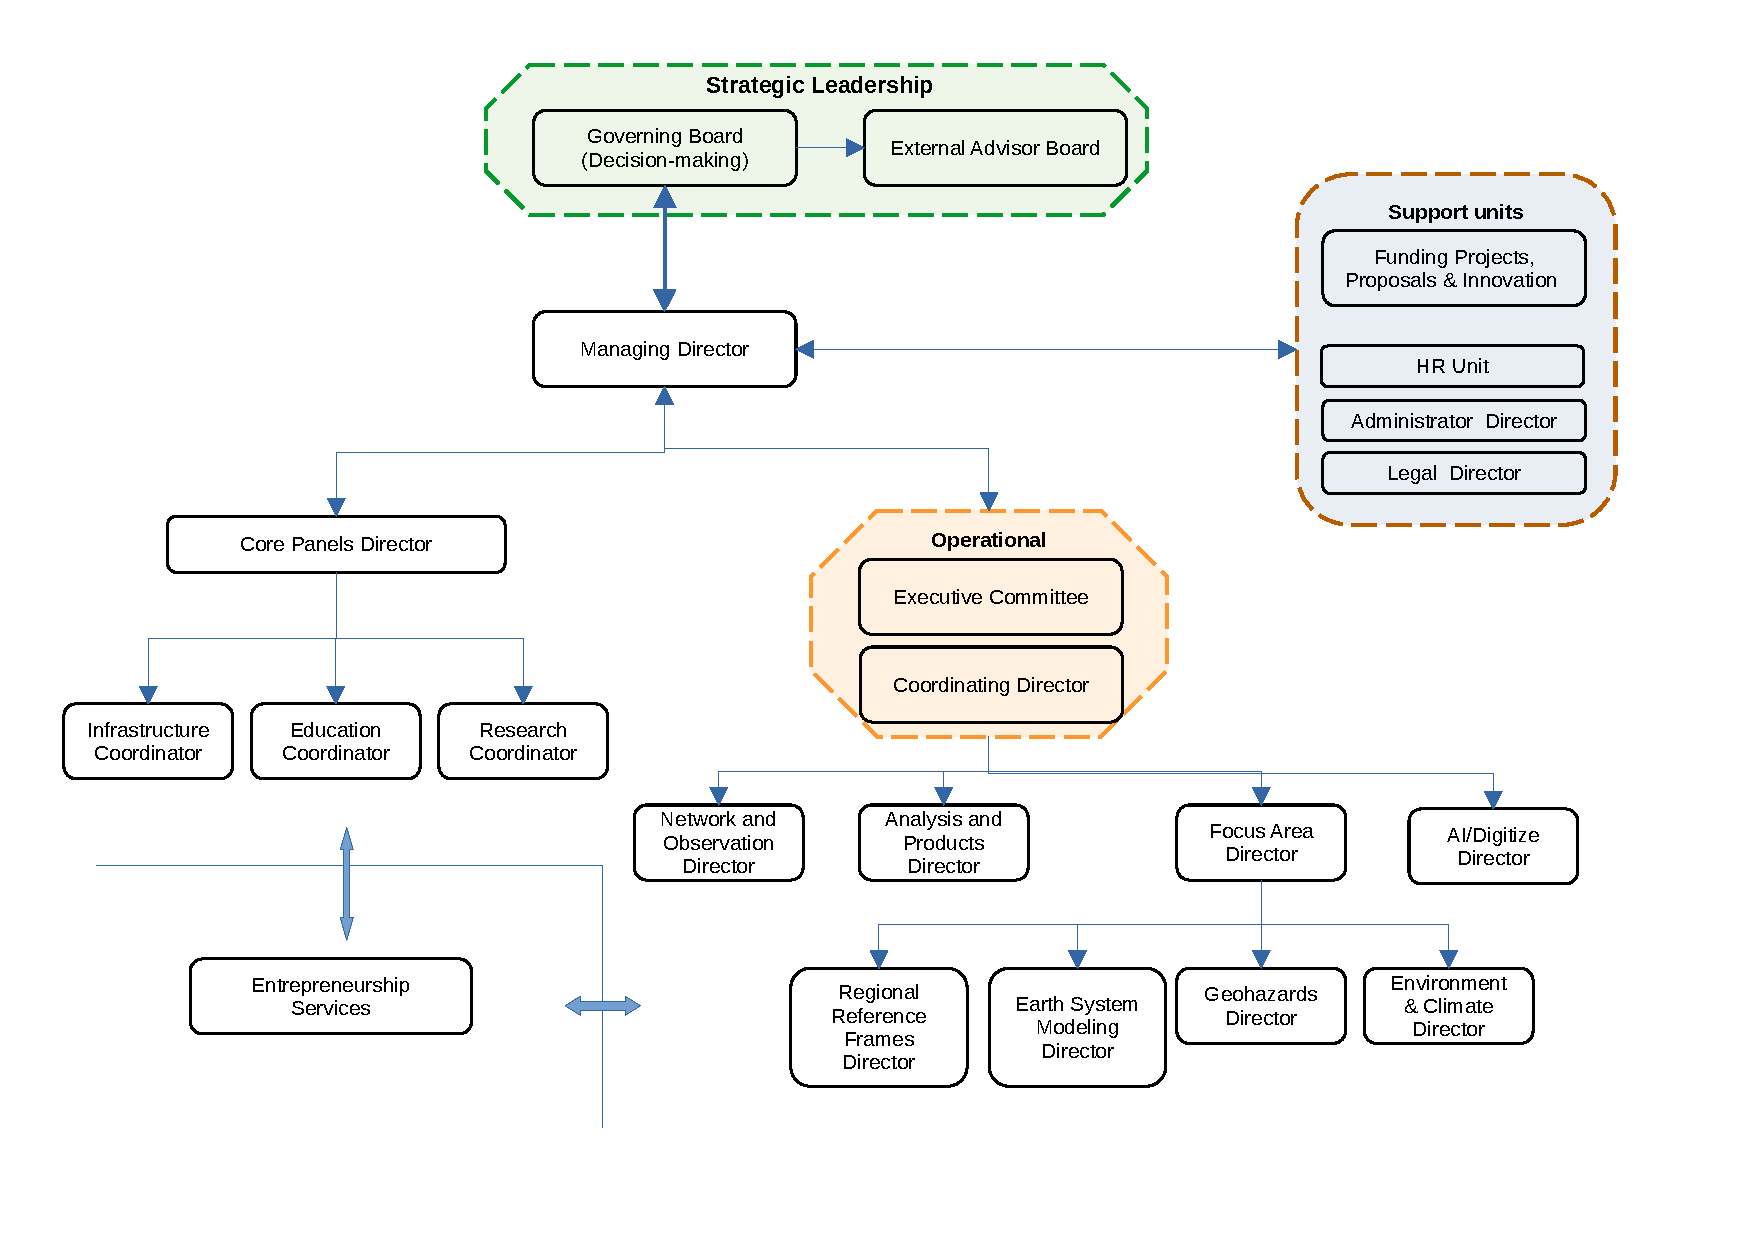
\includegraphics[width=\textwidth]{../Structure_draft3.pdf}
\end{frame}

\begin{frame}{Proposal Writting}
Sustainable Innovations will help with proposal writting and submission. The bulk of the work will be done by NTUA.
\centering
\includegraphics[width=\textwidth]{../payment_options.png}
\end{frame}

% Slide 3
%\begin{frame}{Conclusion}
%  \begin{block}{Contact}
%    Email: yourname@example.com
%  \end{block}
%\end{frame}

\end{document}

